\documentclass[11pt]{article}
\usepackage[utf8]{inputenc}
\usepackage[english]{babel}
\usepackage[font=small,labelfont=bf]{caption}
\usepackage{geometry}
\usepackage[sort&compress, numbers, super]{natbib}
\usepackage{pxfonts}
\usepackage{graphicx}
\usepackage{setspace}
\usepackage{hyperref}
\usepackage{lineno}

\newcommand{\argmax}{\mathop{\mathrm{argmax}}\limits}

\newcommand{\dynamicsRandom}{S1}
\newcommand{\dynamicsAdaptive}{S2}
\newcommand{\accuracyByList}{S3}
\newcommand{\clusterCorrs}{S4}
\newcommand{\fingerprintsRandom}{S5}
\newcommand{\fingerprintsAdaptive}{S6}
\newcommand{\recallInit}{S7}
\newcommand{\fingerprintTrajectoryRandom}{S8}

\doublespacing
\linenumbers

\title{Carryover effects in free recall reveal how prior experiences influence memories of new experiences}
\author{Jeremy R. Manning\textsuperscript{1, *}, Andrew C. Heusser\textsuperscript{1, 2}, Kirsten Ziman\textsuperscript{1, 3},\\Emily Whitaker\textsuperscript{1}, and Paxton C. Fitzpatrick\textsuperscript{1}\\\textsuperscript{1}Dartmouth College\\\textsuperscript{2}Akili Interactive\\\textsuperscript{3}Princeton University\\\textsuperscript{*}Corresponding author: jeremy.r.manning@dartmouth.edu}

\date{}

\begin{document}
\maketitle

\begin{abstract} We perceive, interpet, and remember ongoing experiences
through the lens of our prior experiences. Inferring that we are one type of
situation versus another can lead us to interpret the same physical experience
differently. In turn, this can affect how we focus our attention, form
expectations of what will happen next, remember what is happening now, draw on
our prior related experiences, and so on. To study these phenomena, we asked
participants to perform simple word list learning tasks. Across different
experimental conditions, we held the set of to-be-learned words constant, but
we manipulated the orders in which the words were studied. We found that these
order manipulations affected not only how the participants recalled the ordered
lists, but also how they recalled later randomly ordered lists. Our work shows
how structure in our ongoing experiences can exert influence on how we remember
unrelated subsequent experiences. \end{abstract}


\section*{Introduction}

% the role of context and prior experience in memory 

Experience is subjective: different people who encounter identical physical
experiences can take away very different meanings and memories. One reason is
that our subjective experiences in the moment are shaped in part the
idiosyncratic prior experiences, memories, goals, thoughts, expectations, and
emotions that we bring with us into the present moment. These factors
collectively define a \textit{context} for our experiences~\citep{Mann20}. %
situation models: forming expectations, predicting ambiguous future experiences
The contexts we encounter help us to construct \textit{situation
models}~\citep{RangRitc12, MannEtal15} or \textit{schemas}~\citep{MasiEtal22,
BaldEtal18} that describe how experiences are likely to unfold based on our
prior experiences with similar contextual cues. For example, when we enter a
sit-down restaurant, we might expect to be seated at a table, given a menu, and
served food. Priming someone to expect a particular situation or context can
also influence how they resolve potentail ambiguities in their ongoing
experiences, including ambiguous movies and narratives~\citep{YeshEtal17}.

% gap between "classic" free recall tasks and naturalistic (or real-world)
% memory tasks 

Our understanding of how we form situation models and schemas, and how they
interact with our subjective experiences and memories, is constrained in part
by substantial differences in how we study these processes. Situation models
and schemas are most often studied using ``naturalistic'' stimuli such as
narratives and movies~\citep{ZwaaEtal95,ZwaaRadv98, NastEtal20}. In contrast,
our understanding of how we organize our memories has been most widely studied
using more traditional paradigms like free recall of random word
lists~\citep{Kaha12}. In free recall, participants study lists of items and are
instructed to recall the items in any order they choose. The orders in which
words come to mind can provide insights into how participants have organized
their memories of the studied words. Because random word lists are unstructured
by design, it is not clear if or how non-trivial situation models might apply
to these stimuli. Nevertheless, there are \textit{some} commonalities between
memory for word lists and memory for real-world experiences.

Like remembering real-world experiences, remembering words on a studied list
requires distinguishing the current list from the rest of one's experience. To
model this fundamental memory capability, cognitive scientists have posited the
existence of a special representation, called \emph{context}, that is
associated with each list. According to early
theories~\citep[e.g.][]{Este55a,AndeBowe72} context representations are
composed of many features which fluctuate from moment to moment, slowly
drifting through a multidimensional feature space. During recall, this
representation forms part of the retrieval cue, enabling us to distinguish list
items from non-list items. Understanding the role of context in memory
processes is particularly important in self-cued memory tasks, such as
\textit{free recall}, where the retrieval cue is ``context'' itself.

Over the past half-century, context-based models have enjoyed impressive
success at explaining many stereotyped behaviors observed during free recall
and other list-learning tasks~\citep{Este55a, RaaiShif80, GlenEtal83,
HowaKaha02a, SiroEtal05, KimbEtal07, PolyKaha08, PolyEtalTulv, SedeEtal08,
PolyEtal09, ShanHowa12}. These phenomena include the well-known recency and
primacy effects (superior recall of items from the end and, to a lesser extent,
from the beginning of the study list), as well as semantic and temporal
clustering effects~\citep{KahaEtal08}. The contiguity effect is an example of
temporal clustering, which is perhaps the dominant form of organization in free
recall. This effect can be seen in the tendency for people to successively
recall items that occupied neighboring positions in the study list. For
example, if a list contained the sub-sequence \textsc{``absence hollow pupil''}
and the participant recalls the word \textsc{``hollow''}, it is far more likely
that the next response will be either \textsc{``pupil''} or
\textsc{``absence''} than some other list item~\citep{Kaha96}. In addition,
there is a strong forward bias in the contiguity effect: subjects make forward
transitions (i.e., \textsc{``hollow''} followed by \textsc{``pupil''}) about
twice as often as they make backward transitions, despite an overall tendency
to begin recall at the end of the list. There are also striking effects of
semantic clustering~\citep{RomnEtal93, Bous53, BousEtal54, JenkRuss52,
MannKaha12}, whereby the recall of a given item is more likely to be followed
by recall of a similar or related item than a dissimilar or unrelated one. In
general, people organize memories for words along a wide variety of stimulus
dimensions. As captured by models like the \textit{Context Maintenance and
Retrieval Model}~\citep{PolyEtal09}, the stimulus features associated with each
word (e.g.\ the word's meaning, font size, font color, location on the screen,
size of the object the word represents, etc.) are incorporated into the
participant's mental context representation~\citep{SmitVela01, MannEtal15,
Mann20, MannEtal11, MannEtal12}. During a memory test, any of these features
may serve as a memory cue, which in turn leads the participant to recall in
succession words that share stimulus features.

% link clustering to schemas...

A key mystery is whether the sorts of situation models and schemas that people
use to organize their memories of real-world experiences might map onto the
clustering effects that reflect how people organize their memories for word
lists. On one hand, situation models and clustering effects both reflect
statistical regularities in ongoing experience. Our memory systems exploit
these regularities when generating inferences about the unobserved past and
yet-to-be-experienced future~\citep{XuEtal22, SchaTurk15, RangRitc12,
BoweEtal79, MomeEtal17}. On the other hand, the rich structure of real-world
experiences and other naturalistic stimuli that enable people to form deep and meaningful
situation models and schemas have no obvious analog in simple word lists.  Often lists
in free recall studies are explicitly \textit{designed} to be devoid of exploitable
temporal structure, for example by sorting the words in a random order~\citep{Kaha12}.

% feature-rich free recall, basic manipulation conditions, preview of findings
We designed an experimental paradigm to explore how people organize their
memories for simple stimuli (word lists) whose temporal properties change
across different ``situations,'' analogous to how the content of real-world
experiences change across different real-world situations. We asked
participants to study and freely recall a series of word lists
(Fig.~\ref{fig:exp}). Across the different conditions in the experiment, we
varied the lists' presentation orders in different ways across lists. The
studied items (words) were designed to vary along three general dimensions:
semantic (word \textit{category}, and physical \textit{size} of the referent),
lexicographic (word \textit{length} and \textit{first letter}), and visual
(font \textit{color} and the onscreen \textit{location} of each word). In our
main manipulation conditions, we asked participants to study and recall eight
lists whose items were sorted by a target feature (e.g., word category). Next,
we asked them to study and recall an additional eight lists whose items had the
same features, but that were sorted in a random temporal order. We were
interested in how these order manipulations affected participants' recall
behaviors on early (sorted) lists, as well as how order manipulations on early
lists affected recall behaviors on later (unsorted) lists. We used a series of
control conditions as a baseline; in these control conditions all of the lists
were sorted randomly, but we manipulated the presence or absence of the visual
features. Finally, in an \textit{adaptive} experimental condition we used
participants' recall behaviors on early lists to manipulate, in real-time, the
presentation orders of subsequent lists. In this adaptive condition, we sought
to identify potential commonalities within and across participants in how
people organized their memories and how those organizational tendancies affect
overall performance.












\section*{Materials and methods}

\subsection*{Participants}

We enrolled a total of 491 Dartmouth undergraduate students across 11
experimental conditions. The conditions included two primary controls (feature
rich, reduced), two secondary controls (reduced (early), reduced (late)), six
order manipulation conditions (category, size, length, first letter, color, and
location), and a final adaptive condition. Each of these conditions are
described in the \textit{Experimental design} subsection below.

Participants received course credit for enrolling in our study. We asked each
participant to fill out a demographic survey that included information about
their self-reported age, gender, ethnicity, race, education, vision, reading
impairments, medications or recent injuries, coffee consumption on the day of
testing, and level of alertness at the time of testing. All components of the
demographics survey were optional. One participant elected not to fill out any
part of the demographic survey, and all other participants report some or all
of their requested demographic information.

We aimed to run (to completion) at least 60 participants in each of the two
primary control conditions and in the adaptive condition. In all other
conditions we set a target enrollment of at least 30 participants. Because our
data collection efforts were coordinated 12 researchers and multiple testing
rooms and computers, it was not feasible for individual experimenters to know
how many participants had been run in each experimental condition until the
relevant databases were synchronized at the end of each working day. We also
over-enrolled participants for each condition to help ensure that we met our
minimum enrollment targets even if some participants dropped out of the study
prematurely or did not show up for their testing session. This led us to exceed
our target enrollments for several conditions.

Participants were assigned to experimental conditions based loosely on their
date of participation. (This aspect of our procedure helped us to more easily
synchronize the experiment databases across multiple testing computers.) Of the
490 participants who opted to fill out the demographics survey, reported ages
ranged from 17 to 31 years (mean: 19.1; standard deviation: 1.356). A total of
318 participants reported their gender as female, 170 as male, and 2
participants declined to report their gender. A total of 442 participants
reported their ethnicity as ``not Hispanic or Latino,'' 39 as ``Hispanic or
Latino,'' and 9 declined to report their ethnicity. Participants reported their
races as White (345 participants), Asian (120 participants), Black or African
American (31 participants), American Indian or Alaska Native (11 particiapnts),
Native Hawaiian or Other Pacific Islander (4 participants), Mixed race (3
participants), Middle Eastern (1 participant), and Arab (1 participant). A
total of 5 participants declined to report their race. We note that several
participants reported more than one of racial category. Participants reported
their highest degrees achieved as ``Some college'' (359 participants), ``High
school graduate'' (117 participants), ``College graduate'' (7 participants),
``Some high school'' (5 participants), ``Doctorate'' (1 participant), and
``Master's degree'' (1 participant). A total of 482 participants reported no
reading impairments, and 8 reported mild reading impairments such as mild
dyslexia. A total of 489 participants reported having normal color vision and 1
participant reported that they were color blind. A total of 482 participants
reported taking no prescription medications and having no recent injuries; 4
participants reported having ADHD, 1 reported having dyslexia, 1 reported
having allergies, 1 reported a recently torn ACL/MCL, and 1 reported a
concussion from several months prior. The participants reported consuming 0 --
3 cups of coffee prior to the testing session (mean: 0.32 cups; standard
deviation: 0.58 cups). Participants reported their current level of alertness,
and we converted their responses to numerical scores as follows: ``very
sluggish'' (-2), ``a little sluggish'' (-1), ``neutral'' (0), ``a little
alert'' (1), and ``very alert'' (2). Across all participants, the full range of
alertness levels were reported (range: -2 -- 2; mean: 0.35; standard deviation:
0.89) .

We dropped from our dataset the 1 participant who reported abnormal color
vision, as well as 39 participants whose data were corrupted due to technical
failures while running the experiment or during the daily database merges. In
total, this left usable data from 452 participants, broken down by experimental
condition as follows: feature rich (67 participants), reduced (61
participants), reduced (late) (41 participants), reduced (early), (42
participants), category (30 participants), size (30 participants), length (30
participants), first letter (30 participants), color (31 participants),
location (30 participants), and adaptive (60 participants). The participant who
declined to fill out their demographic survey participated in the location
condition, and we verified verbally that they had normal color vision.




\subsection*{Experimental design}

Our experiment is a variant of the classic free recall paradigm that we term
\textit{feature-rich free recall}. In feature-rich free recall, participants
study 16 lists, each comprised of 16 words that vary along a number of stimulus
dimensions: semantic category, object size, text color, text location, word
length, and starting letter (Fig.~\ref{fig:exp}). Each list contains four words
from each of four different semantic categories and two object sizes; all other
stimulus features are randomized. After studying each list, the participant
attempts to recall as many words as they can from that list, in any order they
choose. Because each individual word is associated with several well-defined
(and quantifiable) features, and because each list incorporates a diverse mix
of feature values along each dimension, this allows us to evaluate
participants' memory fingerprints in rich detail.

\begin{figure} 
    \centering
        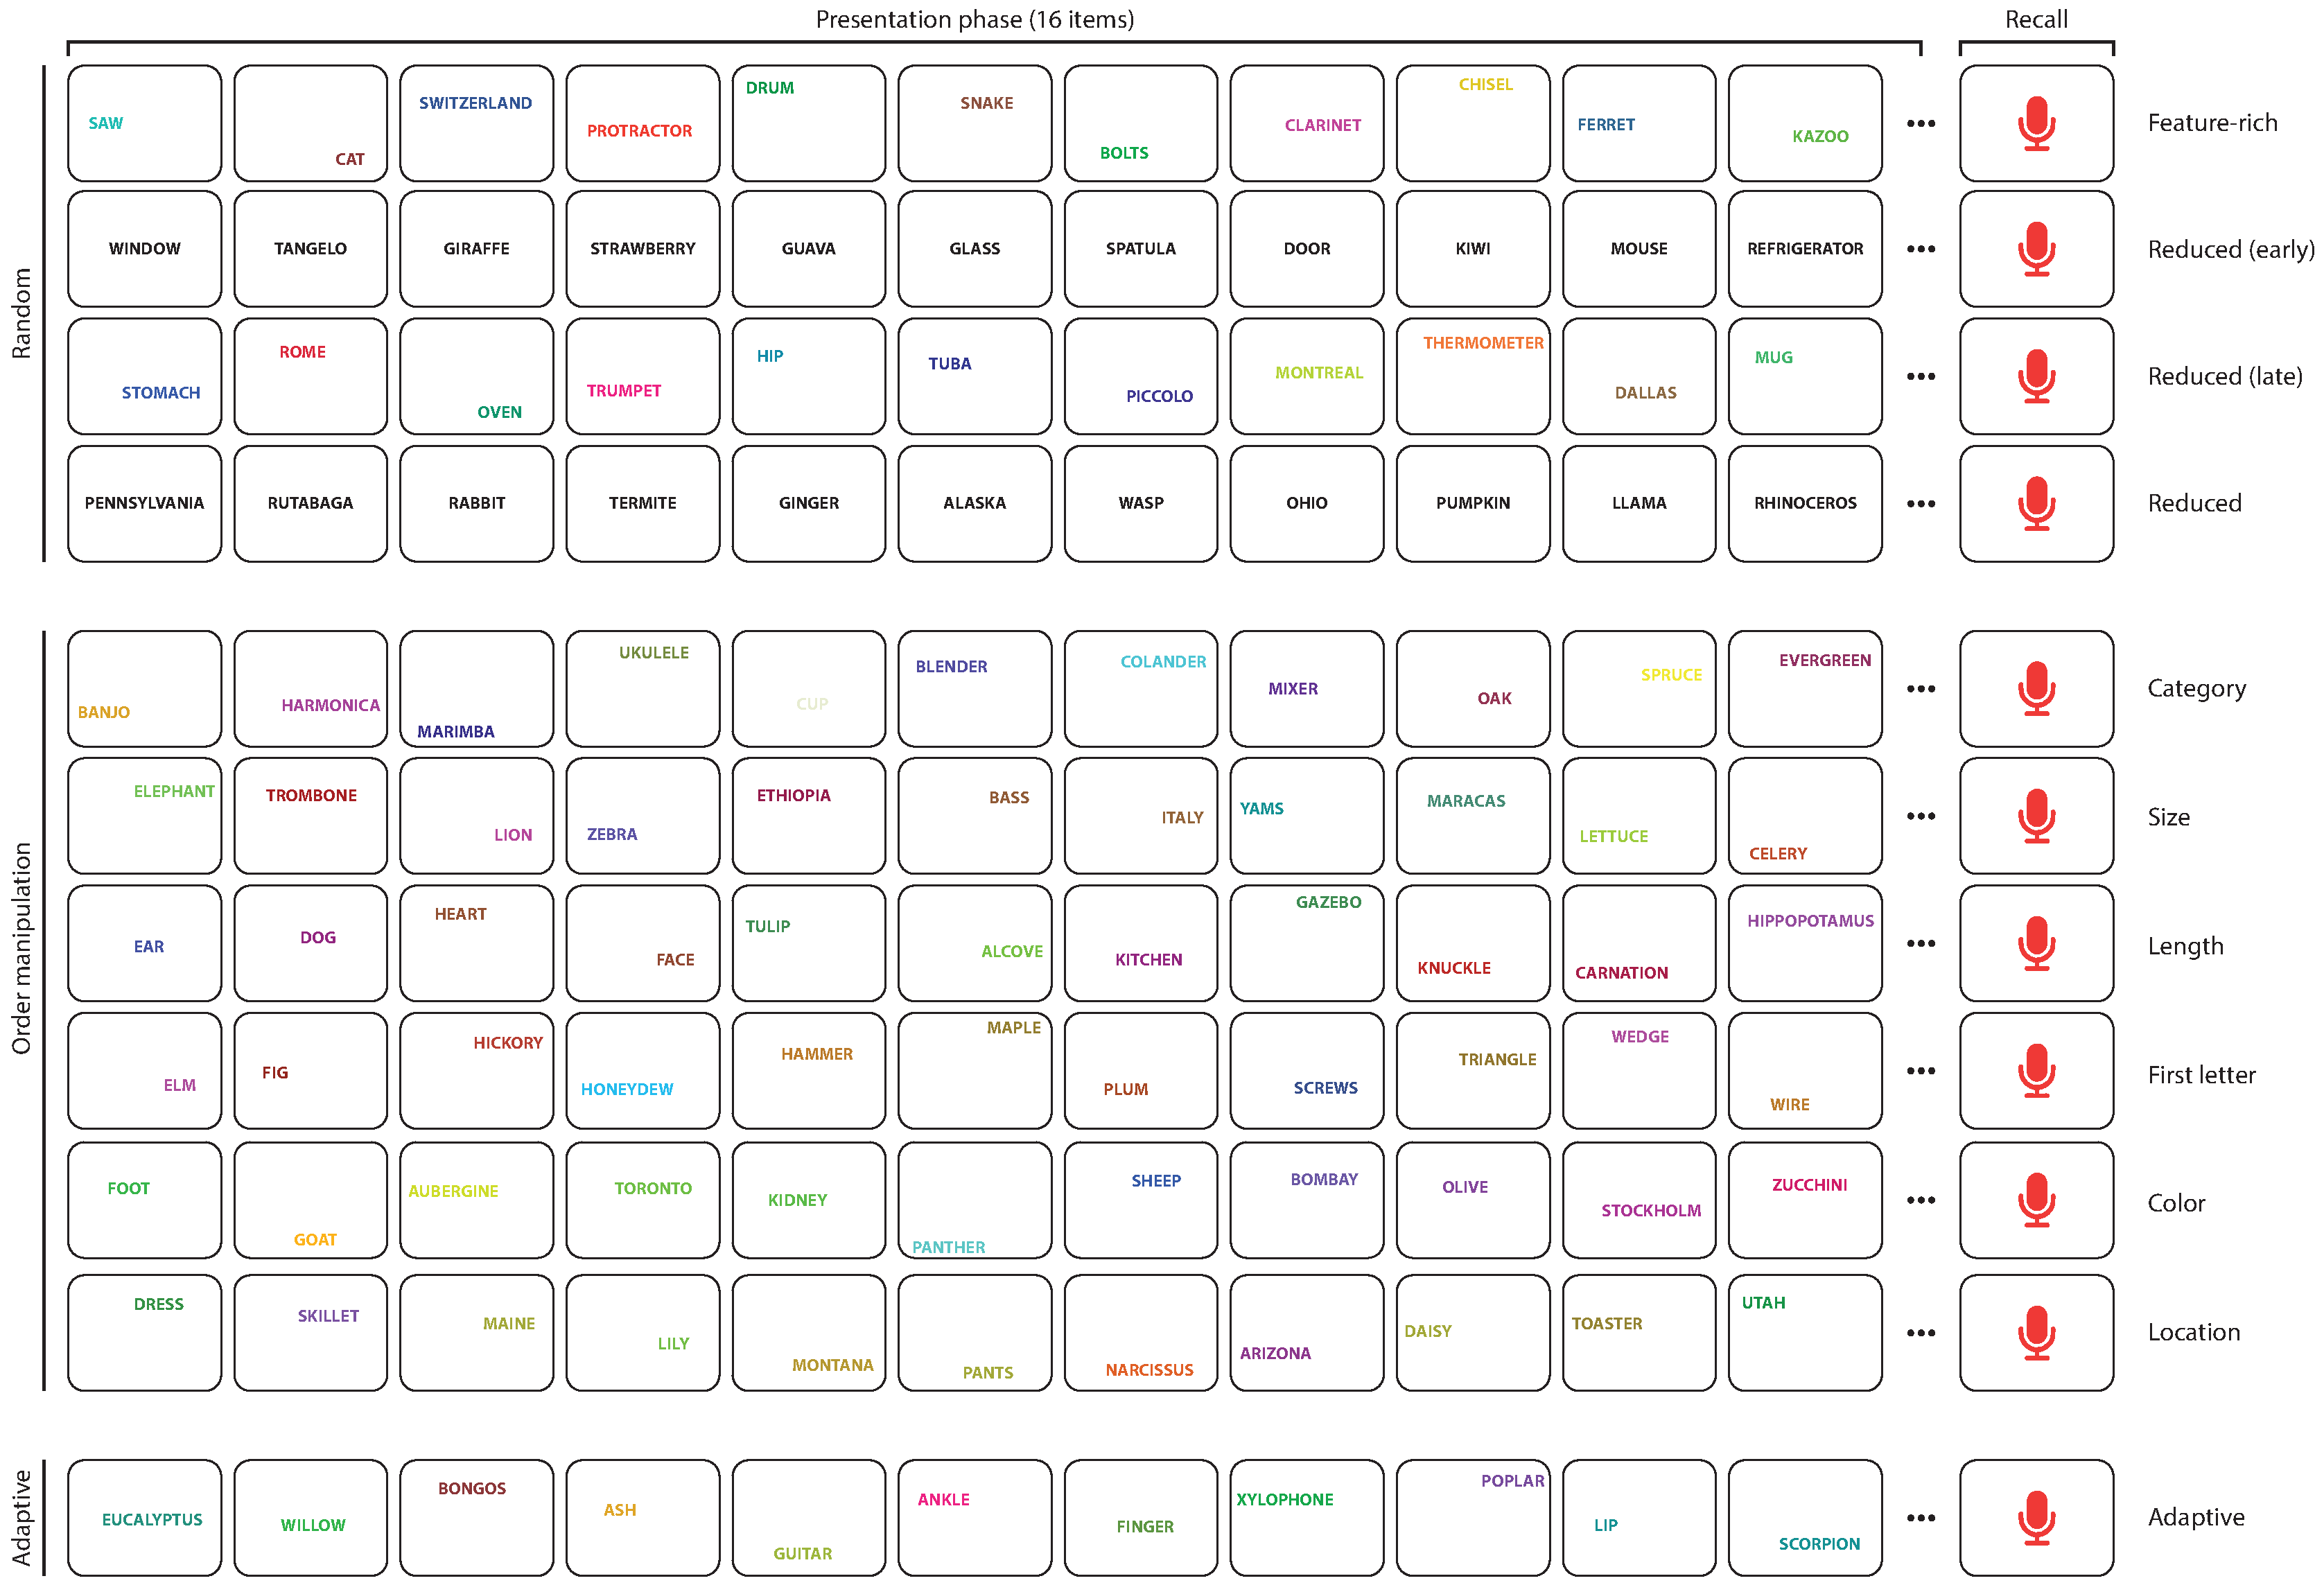
\includegraphics[width=0.75 \textwidth]{figures/FRFR}
        
        \caption{\textbf{Feature-rich free recall.} After studying lists
comprised of words that vary along several feature dimensions, participants
verbally recall words in any order (microphone icon).}

    \label{fig:exp}
\end{figure}



\subsubsection*{Stimuli}

Stimuli in our paradigm were 256 English words selected in a previous
study~\citep{ZimaEtal18}. The words all referred to concrete nouns, and were
chosen from 15 unique semantic categories: body parts, building-related,
cities, clothing, countries, flowers, fruits, insects, instruments,
kitchen-related, mammals, (US) states, tools, trees, and vegetables. We also
tagged each word according to the approximate size of the object the word
referred to. Words were labeled as ``small'' if the corresponding object was
likely able to ``fit in a standard shoebox'' or ``large'' if the object was
larger than a shoebox. Semantic categories varied in how many object sizes they
reflected (mean number of different sizes per category: 1.33; standard
deviation: 0.49). The numbers of words in each semantic category also varied
from 12 -- 28 (mean number of words per category: 17.07; standard deviation
number of words: 4.65). We also identified lexicographic features for each
word, including the words' first letters and lengths (i.e., number of letters).
Across all categories, all possible first letters were represented except for
`Q' (average number of unique first letters per category: 11; standard
deviation: 2 letters). Word lengths ranged from 3 -- 12 letters (average: 6.17
letters; standard deviation: 2.06 letters).

We assigned the categorized words into a total of 16 lists with several
constraints. First, we required that each list contained words from exactly 4
unique categories, each with exactly 4 examplars from each category. Second, we
required that (across all words on the list) at least one instance of both
object sizes were represented. On average, each category was represented in
4.27 lists (standard deviation: 1.16 lists). Aside from these two constraints,
we assigned each word to a unique list. After random assignment, each list
contained words with an average of 11.13 unique starting letters (standard
deviation: 1.15 letters) and an average word length of 6.17 letters (standard
deviation: 0.34 letters).

The above assignments of words to lists was performed once across all
participants, such that every participant studied the same set of 16 lists. We
randomized the study order of these lists across participants. For participants
in some conditions, on some lists, we also randomly varied two additional
visual features to each word: the presentation font color, and the word's
onscreen location. These attributes were assigned independently for word (and
for every participant) at the times the words were displayed onscreen. These
visual features were varied for words in all lists and conditions except for
the ``reduced'' condition (all lists), the first eight lists of the ``reduced
(early)'' condition, and the last eight lists of the ``reduced (late)''
condition. In these latter cases, words were all presented in black at the
center of the experimental computer's display.

To assign a random font color to each word, we selected three integers
uniformly and at random between 0 and 255, corresponding to the red (r), green
(g), and blue (b) color channels for that word. To assign random presentation
locations to each word, we selected two floating point numbers uniformly at
random (one for the word's horizontal $x$ coordinate and the other for its
vertical $y$ coordinate).  The bounds of these coordinates were selected to cover the entire
visible area of the display without cutting off any part of the words.  The words were shown
on 27~in (diagonal) Retina 5K iMac displays (resolution: 5120 $\times$ 2880 pixels).


\subsubsection*{Real-time speech-to-text processing}

Our experimental paradigm incorporates the Google Cloud Speech API
speech-to-text engine~\citep{HalpEtal16} to automatically transcribe
participants' verbal recalls into text. This allows recalls to be transcribed
in real time-- a distinguishing feature of the experiment; in typical verbal
recall experiments the audio data must be parsed manually. In prior work, we
used a similar experimental setup (equivalent to the ``reduced'' condition in
the present study) to verify that the automatically transcribed recalls were
sufficiently close to human-transcribed recalls to yield reliable
data~\citep{ZimaEtal18}. This real-time speech processing component of the
paradigm plays an important role in the ``adaptive'' condition of the
experiment, as described below.

\subsubsection*{Order manipulation conditions}

\paragraph{Feature dimensions.}

\paragraph{Constructing feature-sorted lists.}

\subsubsection*{Random conditions}

\subsubsection*{Adaptive conditions}

\paragraph{Online ``fingerprint'' analysis.}

\paragraph{Ordering ``stabilize'' lists by an estimated fingerprint.}

\paragraph{Ordering ``destabilize'' lists by an estimated fingerprint.}

\subsection*{Analysis}

\subsubsection*{Probability of first recall and probability of $n$\textsuperscript{th} recall}

\subsubsection*{Lag conditional response probability}

\subsubsection*{Computing clustering scores and memory fingerprints}

\subsubsection*{Identifying event boundaries}

\subsubsection*{Serial position curves and recall accuracy}

\subsubsection*{Computing low-dimensional embeddings of memory fingerprints}

\section*{Results}




\begin{figure}[tp] \centering
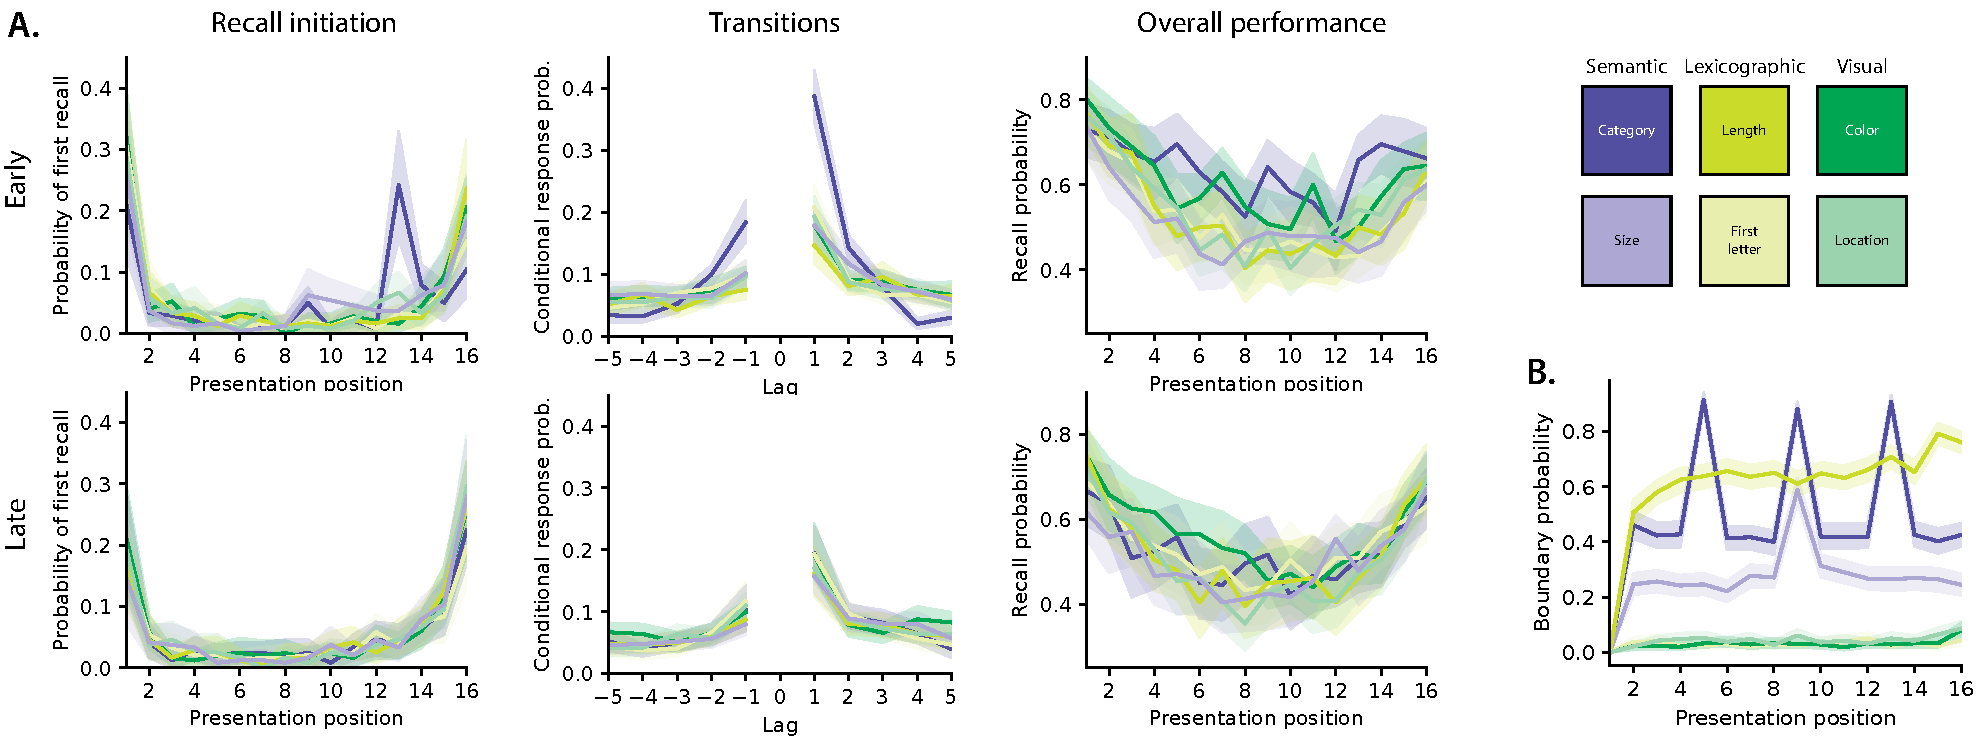
\includegraphics[width=\textwidth]{figures/recall_dynamics}

\caption{\textbf{Recall dynamics in feature rich free recall (order
manipulation conditions).} \textbf{A.} Behavioral plots. \textbf{Left panels.}
The probabilities of initiating recall with each word are plotted as a function
of presentation position. \textbf{Middle panels.} The conditional probabilities
of recalling each word are plotted as a function of the relative position (Lag)
to the words recalled just-prior. \textbf{Right panels.} The overall
probabilities of recalling each word are plotted as a function of presentation
position. \textbf{All panels.} Error ribbons denote bootstrap-estimated 95\%
confidence intervals (calculated across participants). Top panels display the
recall dynamics for early (order manipulation) lists in each condition (color).
Bottom panels display the recall dynamics for late (randomly ordered) lists.
See Figures~\dynamicsRandom~and~\dynamicsAdaptive~for analogous plots for the
random (control) and adaptive conditions. \textbf{B.} Proportion of event
boundaries (see \textit{Methods}) for each condition's feature of focus,
plotted as a function of presentation position.}

    \label{fig:recall-dynamics}
\end{figure}

% figure: accuracy by list
Figure~\accuracyByList.

% figure: recall initiation
Figure~\recallInit.

% figure: clustering effects
\begin{figure}[tp] \centering
    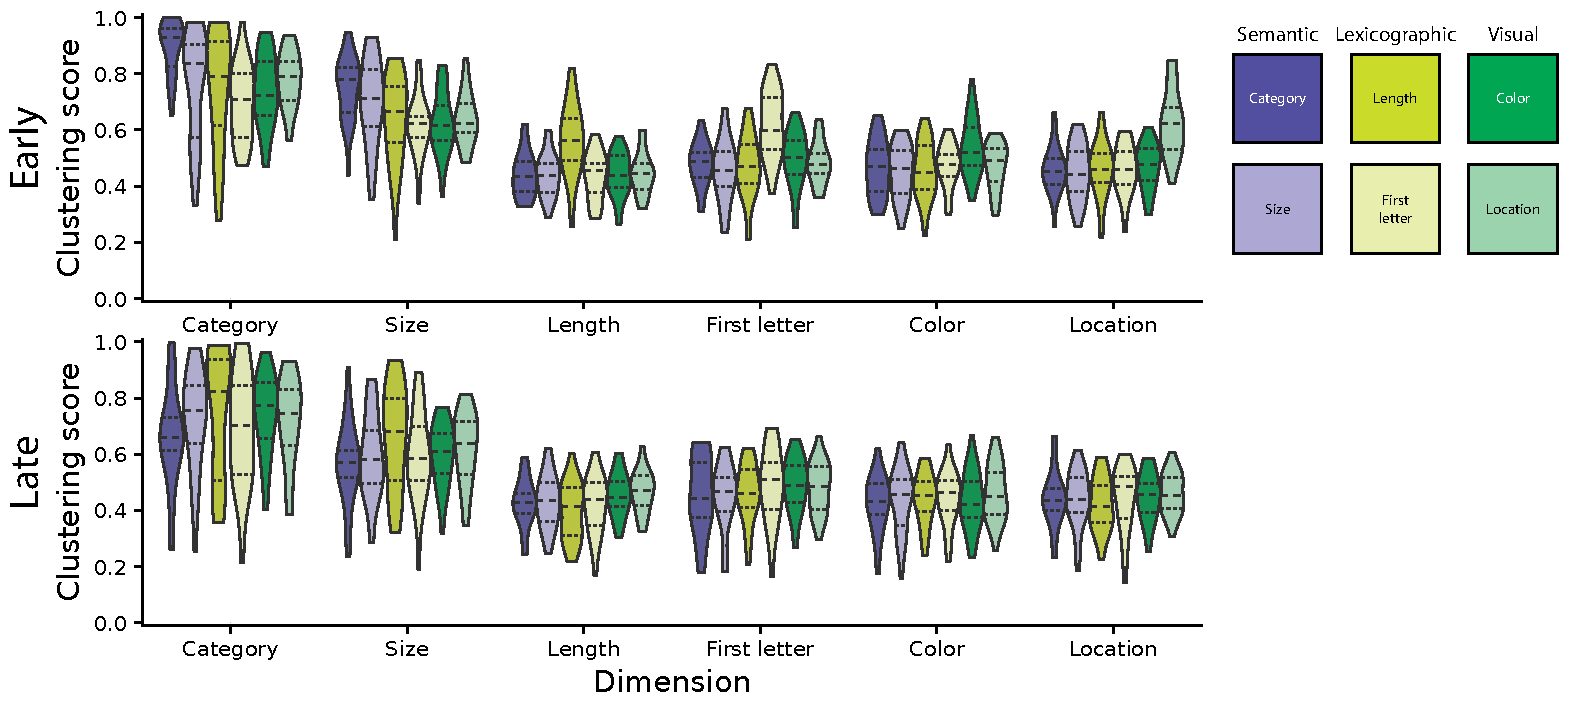
\includegraphics[width=\textwidth]{figures/fingerprints}
    
    \caption{\textbf{Memory ``fingerprints'' (order manipulation conditions).}
    The across-participant distributions of clustering scores for each feature
    type ($x$-coordinate) are displayed for each experimental condition
    (color), separately for order manipulation (early, top) and randomly
    ordered (late, bottom) lists. See
    Figures~\fingerprintsRandom~and~\fingerprintsAdaptive~for analogous plots
    for the random (control) and adaptive conditions.}
        \label{fig:fingerprints}
    \end{figure}

% figure: correlations between clustering scores
Figure~\clusterCorrs.





% figure: feature clustering vs. accuracy, feature clustering vs. temporal clustering
\begin{figure}[tp] \centering
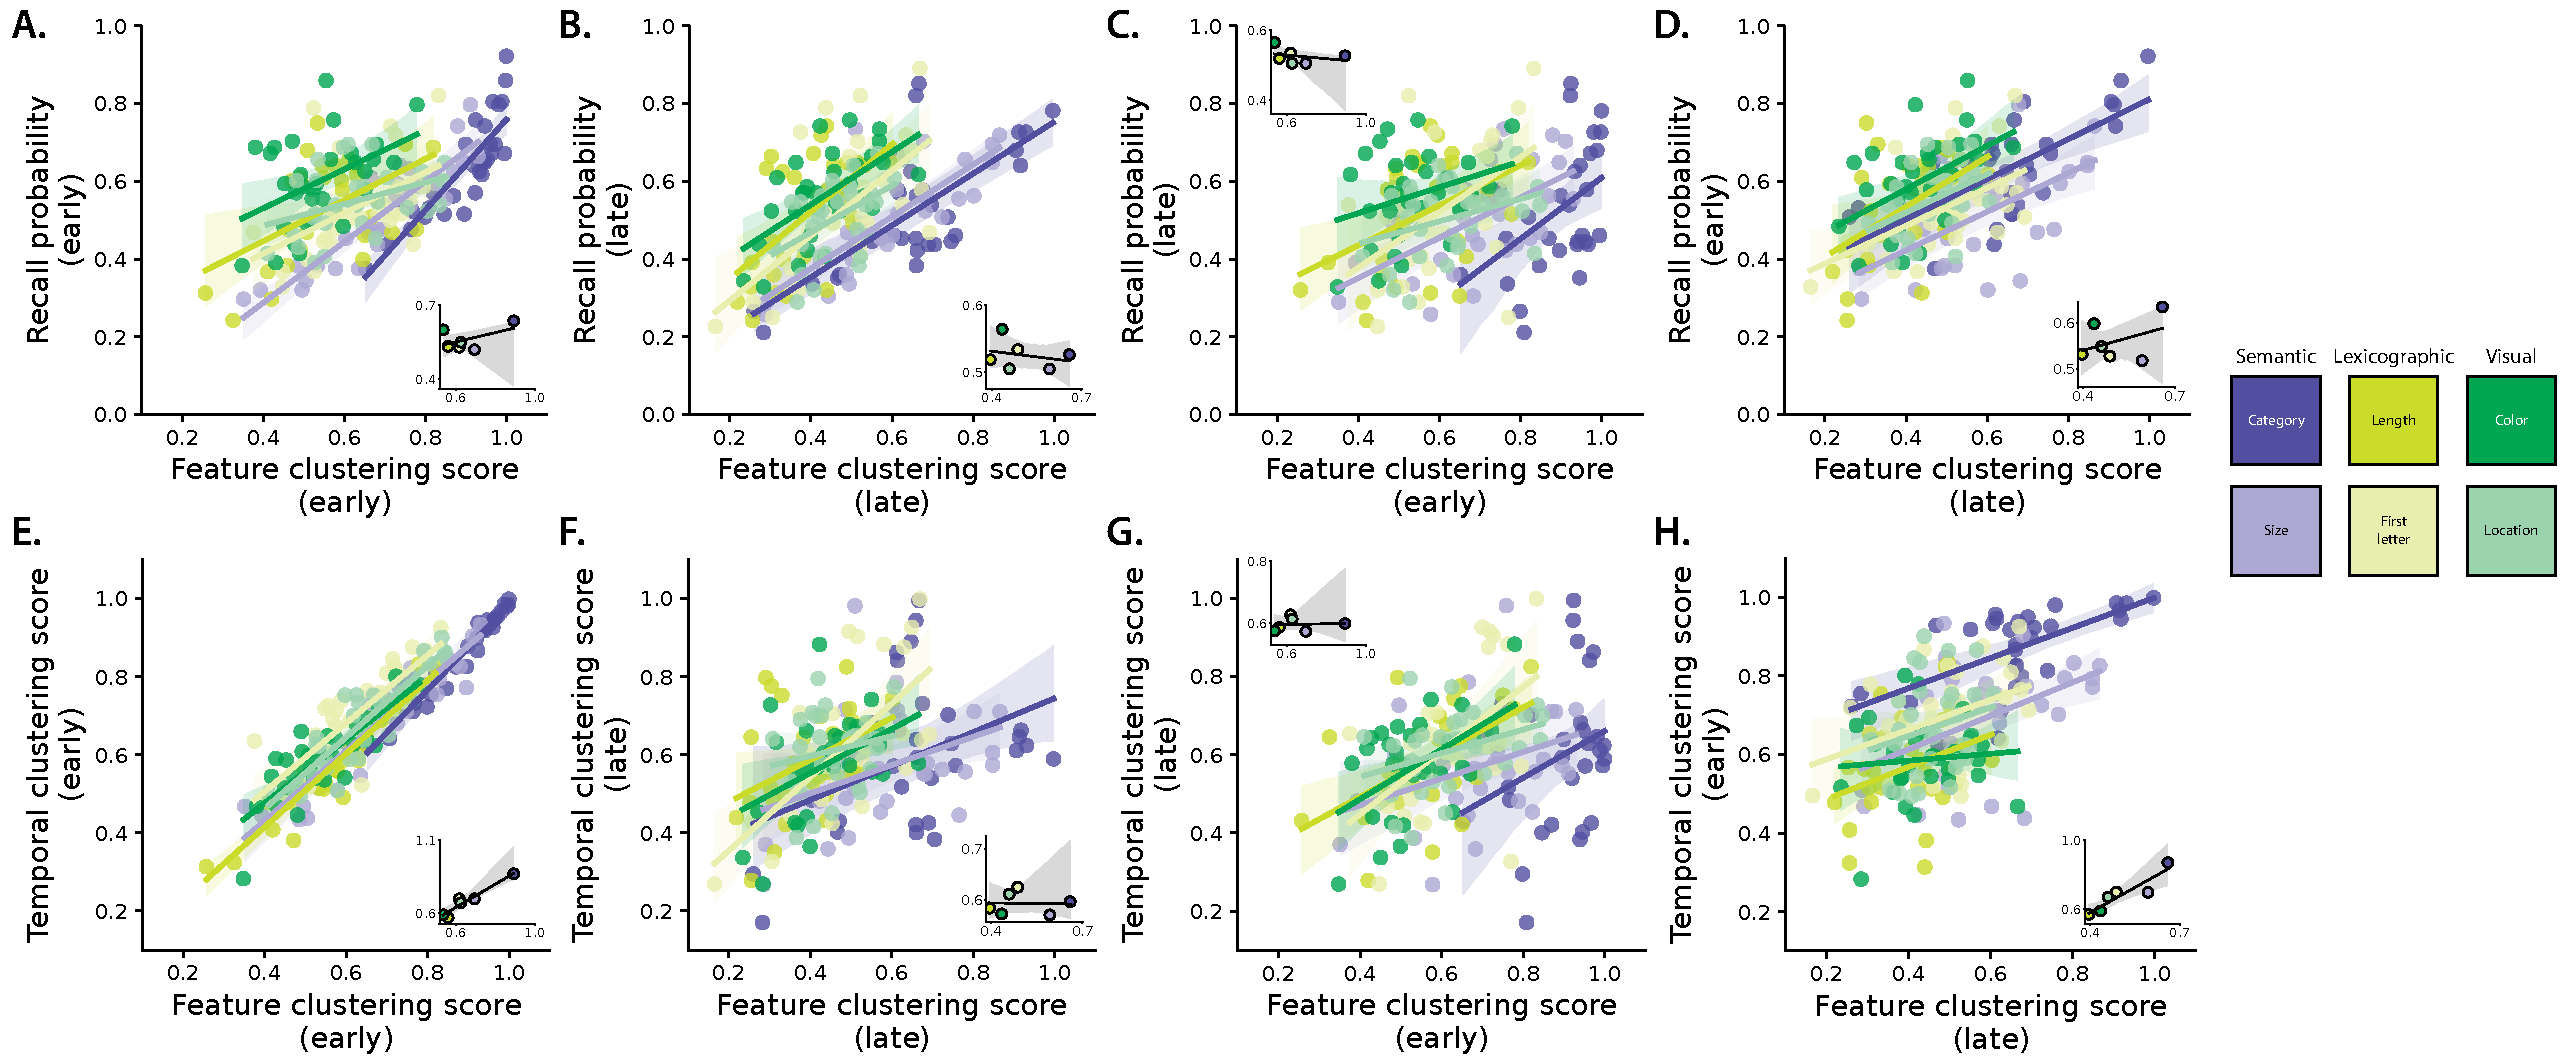
\includegraphics[width=\textwidth]{figures/feature_clustering_vs_accuracy_and_contiguity}

\caption{\textbf{Interactions between feature clustering, recall probability,
and contiguity.} \textbf{A.} Recall probability versus feature clustering
scores for order manipulation (early) lists. \textbf{B.} Recall probability
versus feature clustering for randomly ordered (late) lists. \textbf{C.} Recall
probability on late lists versus feature clustering on early lists. \textbf{D.}
Recall probability on early lists versus feature clustering on late lists.
\textbf{E.} Temporal clustering scores (contiguity) versus feature clustering
scores on early lists. \textbf{F.} Temporal clustering scores versus feature
clustering scores on late lists. \textbf{G.} Temporal clustering scores on late
lists versus feature clustering scores on early lists. \textbf{H.} Temporal
clustering scores on early lists versus feature clustering scores on late
lists. \textbf{All panels.} Each dot in the main scatterplots denotes the
average scores for one participant. The colored regression lines are computed
across participants. The inset displays condition-averaged results, where each
dot reflects a single condition and the regression line is computed across
experimental conditions. All error ribbons denote bootstrap-estimated 95\%
confidence intervals.} \label{fig:clustering-scatterplots} 

\end{figure}


% figure: fingerprint trajectories
\begin{figure}[tp] \centering
    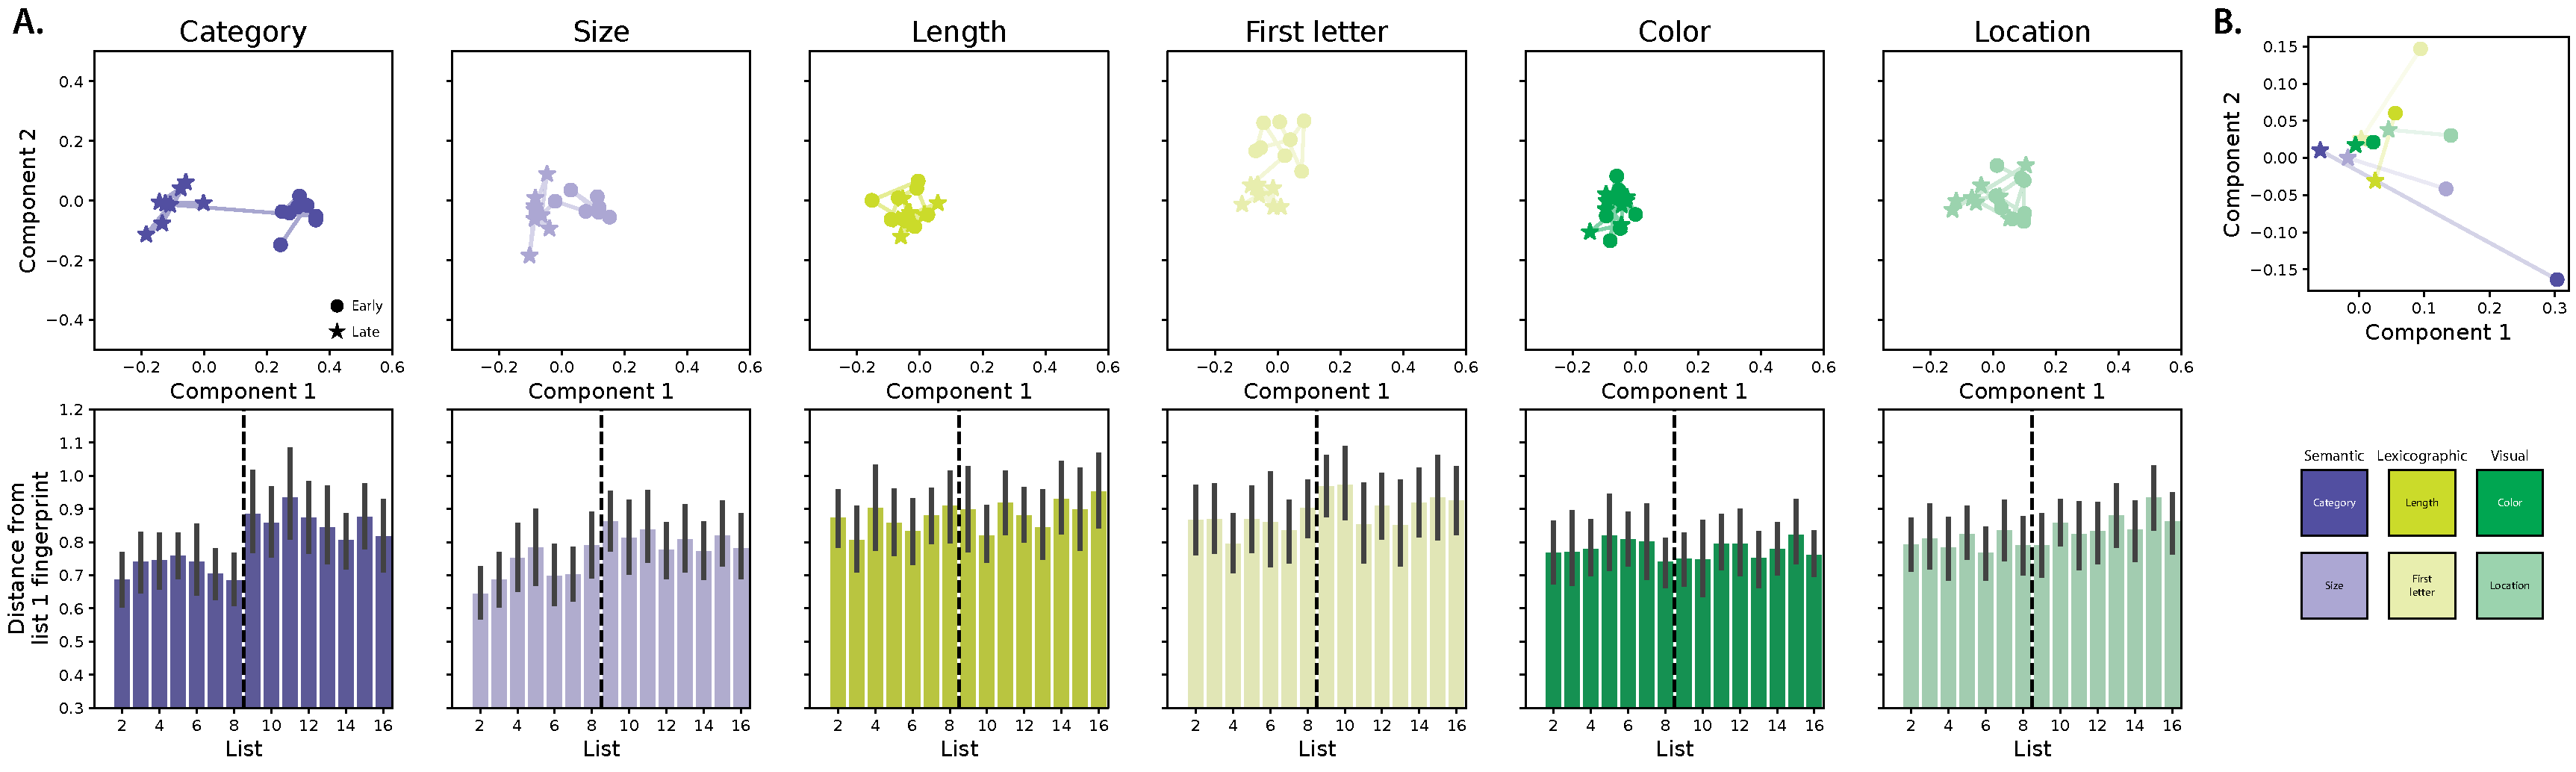
\includegraphics[width=\textwidth]{figures/fingerprint_trajectories}
    
    \caption{\textbf{Memory fingerprint dynamics (order manipulation
    conditions).} \textbf{A.} Each column (and color) reflects an experimental
    condition. In the top panels, each marker displays a 2D projection of the
    (across-participant) average memory fingerprint for one list. Order
    manipulation (early) lists are denoted by circles and randomly ordered
    (late) lists are denoted by stars. All of the fingerprints (across all
    conditions and lists) are projected into a common space. The bar plots in
    the bottom panels display the Euclidean distances of the per-list memory
    fingerprints to the list 0 fingerprint, for each condition. Error bars
    denote bootstrap-estimated 95\% confidence intervals. The dotted vertical
    lines denote the boundaries between early and late lists. \textbf{B.} In
    this panel, the fingerprints for early (circle) and late (star) lists are
    averaged across lists and participants before projecting the fingerprints
    into a (new) 2D space. See Figure~\fingerprintTrajectoryRandom~for
    analogous plots for the random (control) conditions. }
    \label{fig:fingerprint-trajectories}
    
    \end{figure}

% figure: carryover effects: 
%  - clustering early vs. clustering late
%  - clustering carryover vs. accuracy difference
%  - clustering carryover vs. temporal clustering differences
\begin{figure}[tp] \centering
    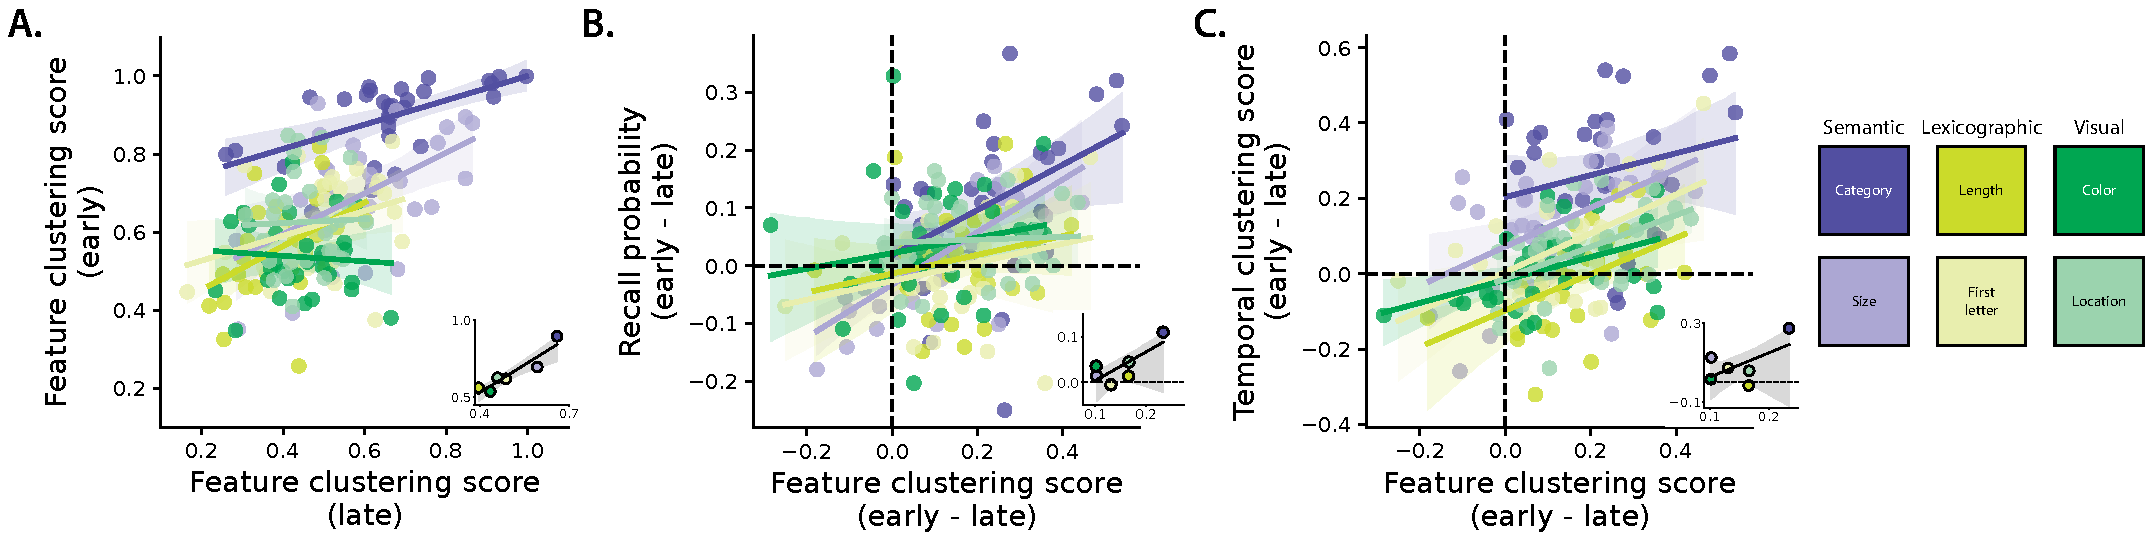
\includegraphics[width=\textwidth]{figures/clustering_carryover}
    
    \caption{\textbf{Feature clustering carryover effects.} \textbf{A.} Feature clustering scores for ordder manipulation (early) versus randomly ordered (late) lists.
    \textbf{B.}  Accuracy differences (on early versus late lists) versus feature clustering ``carryover'' (defined as the differences between the average clustering scores on early and late lists).
    \textbf{C.}  Temporal clustering differences (on early versus late lists) versus feature clustering carryover.  \textbf{All panels.} Each dot in the main scatterplots denotes the
    average scores for one participant. The colored regression lines are computed
    across participants. The inset displays condition-averaged results, where each
    dot reflects a single condition and the regression line is computed across
    experimental conditions. All error ribbons denote bootstrap-estimated 95\%
    confidence intervals.} \label{fig:clustering-carryover}
    \end{figure}

\begin{figure} 
    \centering

    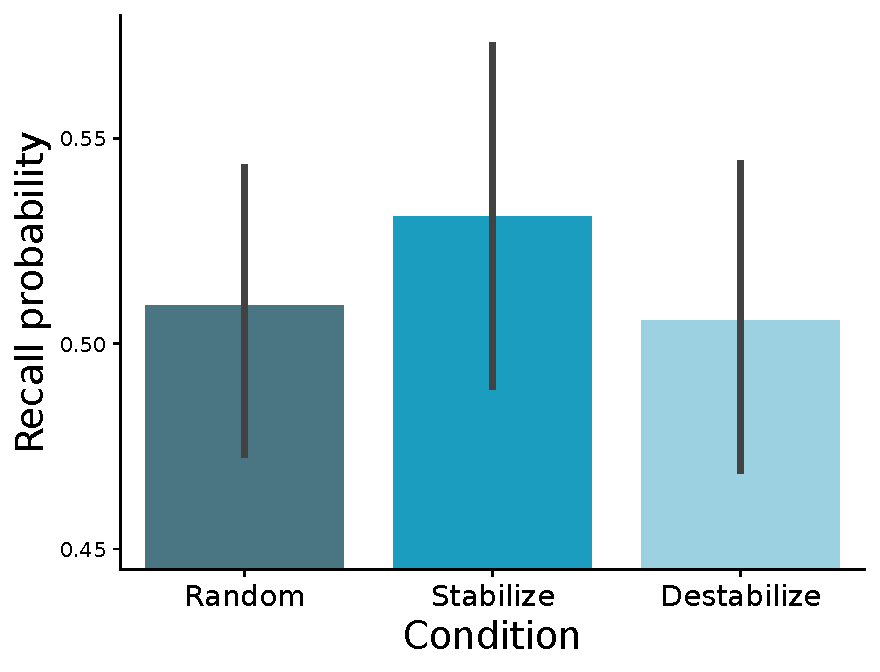
\includegraphics[width=0.4 \textwidth]{figures/source/accuracy_adaptive}
        
        \caption{\textbf{Recall performance (adaptive conditons).} The bars display the average probability of recall (taken across words, lists, and participants)
        for lists from each adaptive condition.  Error bars denote bootstrap-estimated 95\% confidence intervals.  For additional details about
        participants' behavior and performance during the adaptive conditions, see Figure~\dynamicsAdaptive.} 

    \label{fig:adaptive}
\end{figure}

\section*{Discussion}

% recap

% connections to prior work: context effects, priming, situation models

% implications for adaptive learning, education and training

\bibliographystyle{apa}
\bibliography{CDL-bibliography/cdl}
\end{document}
